\chapter{Modulation}

\section{Introduction}
Modulation is done when message signal is not capable of propagating long distance, we change the signal by multiplying another high frequency signal and send the modulated signal.

\par If the characteristics of the message signal is changed, the message contained in it also alters. Hence, is must be ensured that the message signal is not altered in anyway. A high frequency signal can travel up to a longer distance, without getting affected by external disturbances. We take the help of such high frequency signal which is called as a carrier signal to transmit our message signal. Such a process is simply called as Modulation.

Modulation is the process of changing the parameters of the carrier signal, in accordance with the instantaneous values of the modulating signal.

\section{Advantages of Modulation}
The antenna used for transmission, had to be very large, if modulation was not introduced. The range of communication gets limited as the wave cannot travel a distance without getting distorted.

Following are some of the advantages for implementing modulation in the communication systems.

\begin{itemize}
  \item Reduction of antenna size
  \item No signal mixing
  \item Increased communication range
  \item Multiplexing of signals
  \item Possibility of bandwidth adjustments
  \item Improved reception quality

\end{itemize}

\section{Types of Modulation}
There are many types of modulations. Depending upon the modulation techniques used, they are classified as shown in the following figure.
\subfile{Lectures/types.tex}

\chapter{Amplitude Modulation \& Demodulation}
In this chapter we will focus on classic analog modulations
\begin{enumerate}
  \item Amplitude Modulation
  \item Angle Modulation
\end{enumerate}
Before we begin our discussion of different analog modulations, it is important to distinguish between communication systems that do not use modulation (\textbf{baseband communications}) and systems that use modulation (\textbf{carrier communications}).

\section{Baseband \& Carrier communication}
The term \textbf{baseband} is used to designate the frequency band of the original message signal from the source.
\begin{enumerate}
  \item \textbf{Baseband communication}
  \newline
  Message signals are directly transmitted without any modification. Because most baseband signals such as audio and video contain significant low-frequency content, they cannot be effectively transmitted over radio (wireless) links. So,dedicated user channels such as wires and coaxial cables are assigned to each user for long distance communication.
  \par Baseband signals will interfere with one another severely since their band overlaps. FDM allow utilization of one channel by signals through modulation and shifting of spectra to nonoverlapping bands.

  \item \textbf{Carrier communication}
  \newline
  Communication that uses modulation to shift the frequency spectrum of a signal is known \textbf{carrier communication}.There are three parts of a \textbf{sinusoidal carrier} :
  \begin{itemize}
    \item Amplitude $A_c$
    \item Frequency $f_c$
    \item Phase $\phi$
  \end{itemize}
  One of these parameters is varied linearly with the baseband signal $m(t)$,in the case of analog modulation. This results in amplitude modulation(AM), frequency modulation(FM),or phase modulation (PM), respectively.\textbf{Amplitude modulation} is \textit{linear} while the latter two types of carrier modulation are similar and \textit{nonlinear} (called \textbf{angle modulation})
\end{enumerate}


\section{Amplitude Modulation (AM)}
In analog modulation, the amplitude of the carrier signal is made to follow that of the modulating signal. Several variants of amplitude modulation are used in practice. They are Double Side Band Suppressed Carrier (DSBSC) Modulation, Single Sideband Suppressed Carrier (SSBSC) Modulation and Vestigial Sideband Amplitude Modulation (VSBAM).

\subsection{Introduction}
Let $m(t)$ denote a signal that contains information to be transmitted. The information can take analog form or digital form. In traditional analog radio broadcast, $m(t)$ would be an audio signal. In digital communication systems, $m(t)$ may be a sequence of pulses that carries binary data. The information-bearing signal $m(t)$ will be called a \textbf{message signal} for convenience. Also, we will assume that $m(t)$ is a \textbf{baseband signal} with bandwidth W Hz.

Let $ c(t) = A_c cos(2\pi f_c t + \phi)$ denote a \textit{sinusoidal carrier wave}, where $A_c$ is the carrier amplitude and $f_c$ is the carrier frequency. We wish to use the carrier wave to carry the message signal, so that the message signal can appropriately be transmitted over a bandpass channel.There are various carrier modulation techniques. Among them, amplitude modulation (AM) is considered the oldest.

\subsection{Amplitude Modulation Principle}
Let the \textit{Fourier Transform} of $m(t)$ is denoted by $M(f)$. To move the frequency response of $m(t)$ to a new frequency band centered at $f_c$Hz, we use the \textit{frequency shifting property}. In other words, all we need to do is to multiply $m(t)$ by a sinusoid of frequency $f_c$ such that
\begin{equation*}
    s_1 (t) = m(t)cos ~ 2\pi f_c t
\end{equation*}
This immediately acheives the basic aim of modulation by moving the signal frequency content to be centered at $f_c$ via
\begin{equation*}
  S_1 (f) =\frac{1}{2} M(f - f_c) + \frac{1}{2} M(f + f_c)
\end{equation*}
This allow changes in the amplitude of the sinusoid $s_1(t)$ to be proportional to the message signal (Amplitude Modulation)

\subsection{Envelope Formation}
The amplitude-modulated wave may be described by the following formula
\begin{equation}
  s(t) = [1 + k_a m(t)] c(t)\\
  = A_c [1 + k a m(t)] cos(2\pi f_c t),
\end{equation}
where $k_a$ is a constant and is called the amplitude sensitivity. Figures \ref{fig:f2}.(a)-(b) gives an illustration
of the AM process. In the illustration of the AM wave in Figure \ref{fig:f2}(b), the constant $k_a$ is adjusted
such that $1 + k_a m(t) \geq 0$ for all t. It is observed that the envelope of the AM wave takes the same
shape as the message signal (more precisely, the waveform $1 + k_a m(t)$). In fact, the idea of AM is
to use the envelope of the modulated wave $s(t)$ to carry the message signal. There is a requirement for AM to operate properly. Specifically, we must have
\begin{equation}
  |k_a m(t)| \leq 1, ~for~ all~ t.
  \label{equ:e3}
\end{equation}
The condition in \ref{equ:e3} implies that $1 + k a m(t) \geq 0$ for all t. Figure \ref{fig:f2}.(c) shows a situation where
$1 + k_a m(t) < 0$ for some t. We see that the envelope of the AM wave now becomes a distorted version of the message signal. This phenomenon is sometimes known as overmodulation, which can
happen when $k_a$ is set too large.

\begin{figure}[h!]
  \centering
  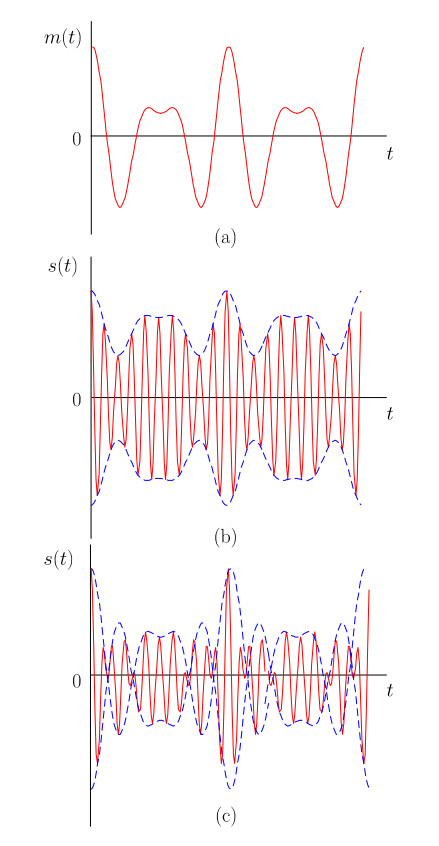
\includegraphics[width = 0.7\textwidth]{figures/AMgraph.png}

  \caption{An illustration of the AM process. (a) The message signal m(t). (b) The AM wave s(t)
when $|k_a m(t)| \leq 1$ holds for all t. (b) The AM wave s(t) when we have $|k_a m(t)| > 1$ for some t.}
  \label{fig:f2}
\end{figure}


We consider several modifications of the previously studied AM scheme, namely, double sideband-suppressed carrier modulation, single sideband modulation and quadrature amplitude modulation.

While the AM scheme is rarely seen in modern communication, we still see some AM concepts,particularly quadrature amplitude modulation, being used—that includes advanced digital com-
munication systems.


\chapter{Double Side-Band Suppressed Carrier}
Recall that m(t) denotes the message signal, and $c(t) = A_c cos(2 \pi f_ct)$ denotes the sinusoidal carrier
wave. Also recall that m(t) is assumed to be a baseband signal with bandwidth W Hz. In double
sideband-suppressed carrier (DSB-SC) modulation, the modulated wave is given by
\begin{equation}
  s(t) = m(t) \cdot c(t) = A_cm(t) cos~w_c t
\end{equation}
If the carrier amplitude $A_c$ is made directly proportional to the modulating signal $m(t)$ then the modulated signal is simply
 $m(t) cos~w_c t$ as shown in Figure \ref{fig:modulation}.
\begin{figure}[h!]

  \tikzset{every picture/.style={line width=0.75pt}} %set default line width to 0.75pt

  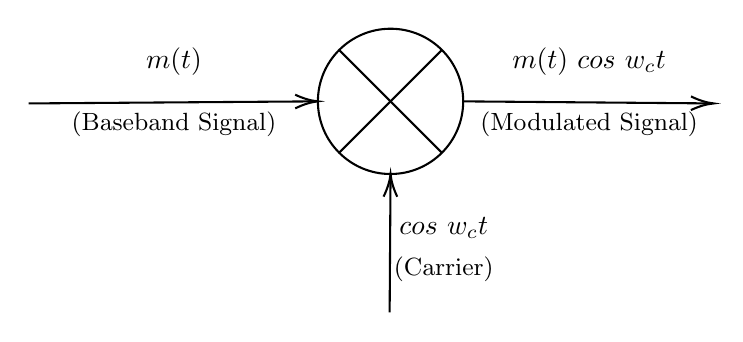
\begin{tikzpicture}[x=0.75pt,y=0.75pt,yscale=-1,xscale=1]
  %uncomment if require: \path (0,471.53334045410156); %set diagram left start at 0, and has height of 471.53334045410156

  \draw    (140,240) -- (277.33,239.01) ;
  \draw [shift={(279.33,239)}, rotate = 539.5899999999999] [color={rgb, 255:red, 0; green, 0; blue, 0 }  ][line width=0.75]    (10.93,-3.29) .. controls (6.95,-1.4) and (3.31,-0.3) .. (0,0) .. controls (3.31,0.3) and (6.95,1.4) .. (10.93,3.29)   ;

  \draw    (349.33,239) -- (468,239.98) ;
  \draw [shift={(470,240)}, rotate = 180.47] [color={rgb, 255:red, 0; green, 0; blue, 0 }  ][line width=0.75]    (10.93,-3.29) .. controls (6.95,-1.4) and (3.31,-0.3) .. (0,0) .. controls (3.31,0.3) and (6.95,1.4) .. (10.93,3.29)   ;

  \draw   (279.33,239) .. controls (279.33,219.67) and (295,204) .. (314.33,204) .. controls (333.66,204) and (349.33,219.67) .. (349.33,239) .. controls (349.33,258.33) and (333.66,274) .. (314.33,274) .. controls (295,274) and (279.33,258.33) .. (279.33,239) -- cycle ; \draw   (289.58,214.25) -- (339.08,263.75) ; \draw   (339.08,214.25) -- (289.58,263.75) ;
  \draw    (313.89,340.69) -- (314.32,276) ;
  \draw [shift={(314.33,274)}, rotate = 450.38] [color={rgb, 255:red, 0; green, 0; blue, 0 }  ][line width=0.75]    (10.93,-3.29) .. controls (6.95,-1.4) and (3.31,-0.3) .. (0,0) .. controls (3.31,0.3) and (6.95,1.4) .. (10.93,3.29)   ;

  \draw (340,300) node   {$cos\ w_{c} t$};
  \draw (210,220) node   {$m( t)$};
  \draw (410,220) node   {$m( t) \ cos\ w_{c} t$};
  \draw (210,250) node  [align=left] {{\small (Baseband Signal)}};
  \draw (410,250) node  [align=left] {{\small (Modulated Signal)}};
  \draw (340,320) node  [align=left] {{\small (Carrier)}};


  \end{tikzpicture}
  \caption{DSB-SC Modulation block Diagram}
  \label{fig:modulation}
\end{figure}
\section{Modulation}
This type of modulation simply shiftsthe spectrum of $m(t)$ to the carrier frequency.Thus, if

\begin{align}
    m(t) &\Longleftrightarrow M(w) \\
    then, ~~~~~~~~~~~~~~~~~~~~~~ m(t)cos~2\pi f_ct & \Longleftrightarrow \frac{1}{2} [ M(f - f_c ) + M(f + f_c )]
\end{align}
Recall that $M(f-f_c)$ is $M(f)$ shifted to the right by $f_c$ and $M(f+f_c)$ is $M(f)$ shifted to the left by $f_c$. Thus the process of modulation shifts the spectrum of the modulating signal to the left and to the right by $f_c$.The Fourier transform of the DSB-SC modulated signal s(t) is given by
\begin{equation}
  \centering
  \begin{split}
    m(t) &\Longleftrightarrow M(w)\\
    M(w) &= \int_{-\infty}^{+\infty} m(t)e^{-jwt} ~dt\\
    We~Know,~~m(t) &= Acos(w_ct + \phi)\\
    Assuming,~A=1 ~and ~Q=0 \\
    m(t) &= cos~w_ct\\
    m(t)cos~w_ct &= \frac{1}{2}(e^{jw_ct} + e^{-jw_ct})m(t)\\
    &= \frac{1}{2}(e^{jw_ct}m(t) + \frac{1}{2}(e^{-jw_ct}m(t)\\
    \therefore M_1(w) &= \frac{1}{2} \int_{-\infty}^{+\infty} e^{jw_ct}m(t)e^{-jwt} ~dt\\
    &= \frac{1}{2} \int_{-\infty}^{+\infty} m(t)e^{-j(w - w_c)t} ~dt\\
    &= \frac{1}{2} \overline{M}(w-w_c)\\
    Similarly, M_2(w) &= \frac{1}{2} \overline{M}(w+w_c)\\
    &m(t)cos~2\pi w_ct \Longleftrightarrow M(w)\\
    M(w) &= \frac{1}{2} [ M(f - f_c ) + M(f + f_c )]\\
  \end{split}
\end{equation}
\begin{align}
  m(t)cos~w_ct &= \frac{1}{2}(e^{jw_ct} + e^{-jw_ct}) m(t)\\
  &= \frac{1}{2}(e^{jw_ct}m(t) + \frac{1}{2}e^{-jw_ct}) m(t)\\
  S(f) &= \frac{A_c}{2} [ M(f - f_c ) + M(f + f_c )]
\end{align}


Figure \ref{fig:DSBSC1} illustrates the corresponding amplitude spectrum. As can be seen in the figure, the
transmission bandwidth of DSB-SC modulation is 2W Hz—the same as the AM transmission
bandwidth.We also observe that the modulated signal spectrum centered at $\pm f_c$ consists of two parts: a portion that lies outside $\pm f_c$, known as the \textit{upper sideband (\textbf{USB})}, and a portion that lies outside $\pm f_c$, known as the \textit{lower sideband (\textbf{LSB})}.
\par Also, the modulated signal does not have any discrete component of the carrier frequency $f_c$. For this reason it is called \textbf{double-sideband suppressed carrier (DSB-SC) modulation}

\begin{figure}
  \centering


\tikzset{every picture/.style={line width=0.75pt}} %set default line width to 0.75pt

\begin{tikzpicture}[x=0.75pt,y=0.75pt,yscale=-1,xscale=1]
%uncomment if require: \path (0,300); %set diagram left start at 0, and has height of 300

\draw  (63,187.63) -- (238.45,187.63)(139.45,51.63) -- (139.45,204.63) (231.45,182.63) -- (238.45,187.63) -- (231.45,192.63) (134.45,58.63) -- (139.45,51.63) -- (144.45,58.63)  ;
\draw    (80.45,149.63) .. controls (142.45,-32.37) and (171.45,220.63) .. (224.45,207.63) ;


\draw  (328.3,191.34) -- (520.97,191.34)(430.3,54.01) -- (430.3,208.63) (513.97,186.34) -- (520.97,191.34) -- (513.97,196.34) (425.3,61.01) -- (430.3,54.01) -- (435.3,61.01)  ;
\draw    (380,190) .. controls (415.63,198.01) and (408.37,69.99) .. (430,70) .. controls (451.63,70.01) and (446.97,200.68) .. (480,190) ;


\draw    (252,130) -- (318,130) ;
\draw [shift={(320,130)}, rotate = 180] [fill={rgb, 255:red, 0; green, 0; blue, 0 }  ][line width=0.75]  [draw opacity=0] (8.93,-4.29) -- (0,0) -- (8.93,4.29) -- cycle    ;
\draw [shift={(250,130)}, rotate = 0] [fill={rgb, 255:red, 0; green, 0; blue, 0 }  ][line width=0.75]  [draw opacity=0] (8.93,-4.29) -- (0,0) -- (8.93,4.29) -- cycle    ;
\draw    (420,70) -- (440,70) ;



\draw (80,100) node   {$m( t)$};
\draw (240,200) node [scale=0.9]  {$t$};
\draw (430,40) node   {$M( f)$};
\draw (380,200) node  [align=left] {\mbox{-}B};
\draw (480,200) node  [align=left] {B};
\draw (450,70) node  [align=left] {2A};
\draw (440,200) node [scale=0.9]  {$0$};


\end{tikzpicture}
  \caption{}
  \label{fig:DSBSC1}
\end{figure}

\begin{figure}[h!]
  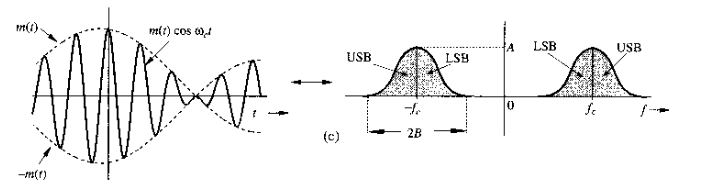
\includegraphics[width = 1.1\textwidth]{figures/DSBSC1.png}
  \caption{}
  \label{fig:DSBSC2}
\end{figure}

The relationshop of $B$ to $f_c$ is of interest. Figure \ref{fig:DSBSC2} shows that $f_c \geq B$, thus avoiding overlap of the modulated spectra centered at $f_c$ and $-f_c$. If $f_c < B$, the the two copies of message spectra overlap and the information of $m(t)$ is lost during modulation, which makes it impossible to get back the m(t) from the modulated signal $m(t)cos~w_ct$.
\par The difference between AM and DSB-SC modulation is that the DSB-SC modulated wave does not
have the pure carrier component. Consequently, one hundred percent of the transmission power is
spent on sending the message signal.

\section{Demodulation}
DSB-SC modulation shifts spectrum to right and left by $f_c$.To recover the original signal m(t) from the modulated signal, it is necessary to retranslate the spectrum to its original position. This process is known as \textbf{demodulation}.
If modulated signal spectrum in Figure \ref{fig:DSBSC2} is
shifted to the left and to the right by $f_c$ and multiplied by
half, we obtain \ref{fig:DSBSC3}

\begin{figure}[h!]
  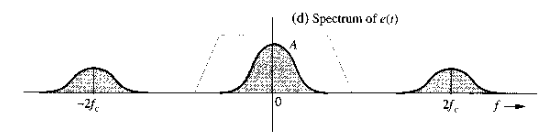
\includegraphics[width = 1.1\textwidth]{figures/DSBSC3.png}
  \caption{}
  \label{fig:DSBSC3}
\end{figure}

The figure contains the desired baseband spectrum plus and unwanted spectrum at $\pm 2f_c$. The unwanted spectrum can be suppressed by a low-pass filter.
\par Demodulation consists of multiplication of the incoming
modulated signal $m(t)cos~w_ct$ by a carrier $cos~w_ct$ followed by a low pass filter.

\begin{figure}[h!]
  \centering

\tikzset{every picture/.style={line width=0.75pt}} %set default line width to 0.75pt

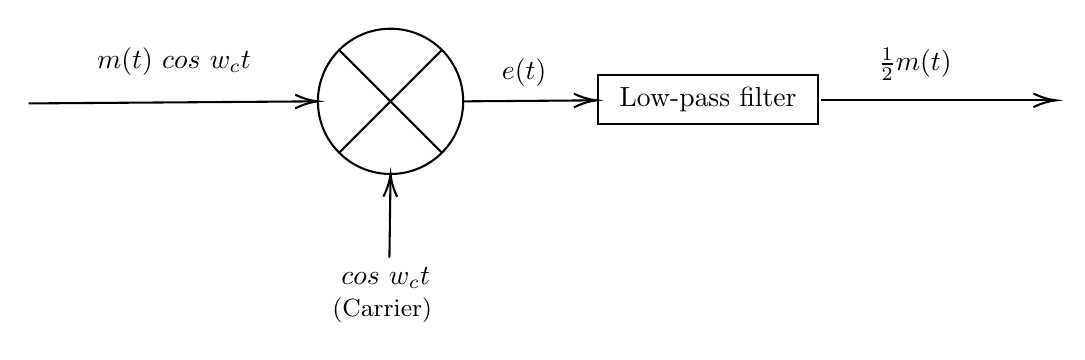
\begin{tikzpicture}[x=0.75pt,y=0.75pt,yscale=-1,xscale=1]
%uncomment if require: \path (0,198.53334045410156); %set diagram left start at 0, and has height of 198.53334045410156

\draw    (138,66) -- (275.33,65.01) ;
\draw [shift={(277.33,65)}, rotate = 539.5899999999999] [color={rgb, 255:red, 0; green, 0; blue, 0 }  ][line width=0.75]    (10.93,-3.29) .. controls (6.95,-1.4) and (3.31,-0.3) .. (0,0) .. controls (3.31,0.3) and (6.95,1.4) .. (10.93,3.29)   ;

\draw    (347.33,65) -- (409.63,64.53) ;
\draw [shift={(411.63,64.51)}, rotate = 539.56] [color={rgb, 255:red, 0; green, 0; blue, 0 }  ][line width=0.75]    (10.93,-3.29) .. controls (6.95,-1.4) and (3.31,-0.3) .. (0,0) .. controls (3.31,0.3) and (6.95,1.4) .. (10.93,3.29)   ;

\draw   (277.33,65) .. controls (277.33,45.67) and (293,30) .. (312.33,30) .. controls (331.66,30) and (347.33,45.67) .. (347.33,65) .. controls (347.33,84.33) and (331.66,100) .. (312.33,100) .. controls (293,100) and (277.33,84.33) .. (277.33,65) -- cycle ; \draw   (287.58,40.25) -- (337.08,89.75) ; \draw   (337.08,40.25) -- (287.58,89.75) ;
\draw    (311.79,140.33) -- (312.31,102) ;
\draw [shift={(312.33,100)}, rotate = 450.77] [color={rgb, 255:red, 0; green, 0; blue, 0 }  ][line width=0.75]    (10.93,-3.29) .. controls (6.95,-1.4) and (3.31,-0.3) .. (0,0) .. controls (3.31,0.3) and (6.95,1.4) .. (10.93,3.29)   ;

\draw    (519.63,64.51) -- (630.97,64.51) ;
\draw [shift={(632.97,64.51)}, rotate = 180] [color={rgb, 255:red, 0; green, 0; blue, 0 }  ][line width=0.75]    (10.93,-3.29) .. controls (6.95,-1.4) and (3.31,-0.3) .. (0,0) .. controls (3.31,0.3) and (6.95,1.4) .. (10.93,3.29)   ;

\draw (310,150) node   {$cos\ w_{c} t$};
\draw (208,46) node   {$m( t) \ cos\ w_{c} t$};
\draw (376.67,51.33) node   {$e( t)$};
\draw (308.33,165.67) node  [align=left] {{\small (Carrier)}};
\draw     (412.27, 52.23) rectangle (518.4, 75.77)   ;
\draw (465.33,64) node  [align=left] {Low-pass filter};
\draw (565,47) node   {$\frac{1}{2} m( t)$};


\end{tikzpicture}

  \caption{DSB-SC Demodulation Block Diagram}
  \label{}
\end{figure}
This can be verified in the time domain by observing $e(t)$
as follows:
\begin{equation}
  e(t) = m(t)cos^2~w_ct\\
      = \frac{1}{2}[m(t)+m(t)cos~2w_ct]
\end{equation}
Therefore, the Fourier transform of the signal $e(t)$ is
\begin{equation}
   E(f) = \frac{1}{2}M(f) + \frac{1}{4}[M(f +2f_c)+M(f-2f_c)]
\end{equation}
Signal $e(t)$ consists of two components $\frac{1}{2}m(t)$ and $\frac{1}{2}m(t)cos~2w_ct$, with their nonoverlapping spectra
The spectrum of the second component, being a
modulated signal with carrier frequency $2f_c$, is centered at $\pm 2f_c$
This component is suppressed by low-pass filter. On the other hand, the desired component $\frac{1}{2}M(f)$, being a low-pass spectrum (centered at f = 0) passes through the filter unharmed, resulting in $\frac{1}{2}m(t)$. We can get rid  of the inconvenient fraction $\frac{1}{2}$ in the output by using a carrier $cos~2w_ct$ instead of $cos~w_ct$
This method of recovering the baseband signal is called synchronous detection or coherent detection where we
use a carrier of exactly the same frequency(same phase) as the carrier used for modulation.
